\section{Hakram}\label{hakram}

Tags: NPC Creatore: Lorenzo Ispirazione: Hart Marjok, ovviamente.

akram

\section{Hakram}\label{hakram-1}

\begin{center}\rule{0.5\linewidth}{0.5pt}\end{center}

\begin{figure}
\centering
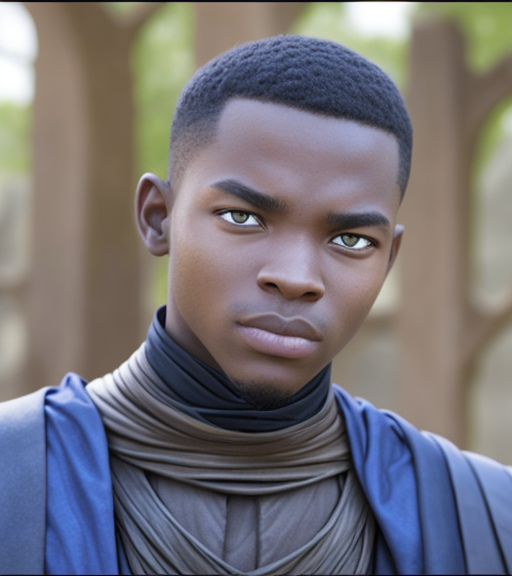
\includegraphics{a-skilled--assassin-ready-to-disappear-with-his-invisibility-cloak-he-is-a-young-black-man-he-is-a_(1).png}
\caption{a-skilled--assassin-ready-to-disappear-with-his-invisibility-cloak-he-is-a-young-black-man-he-is-a
(1).png}
\end{figure}

Informazioni Generali

Età: 27

Data di nascita: 1997

Luogo di nascita: Foresta dei Giganti

Razza: Mezz'elfo

Classe: Ladro

Alleati:

Nemesi: Impero Dishartiano

Alias:

Professione: Ladro

\begin{center}\rule{0.5\linewidth}{0.5pt}\end{center}

\subsection{1. Descrizione Generale}\label{descrizione-generale}

\begin{center}\rule{0.5\linewidth}{0.5pt}\end{center}

\begin{figure}
\centering
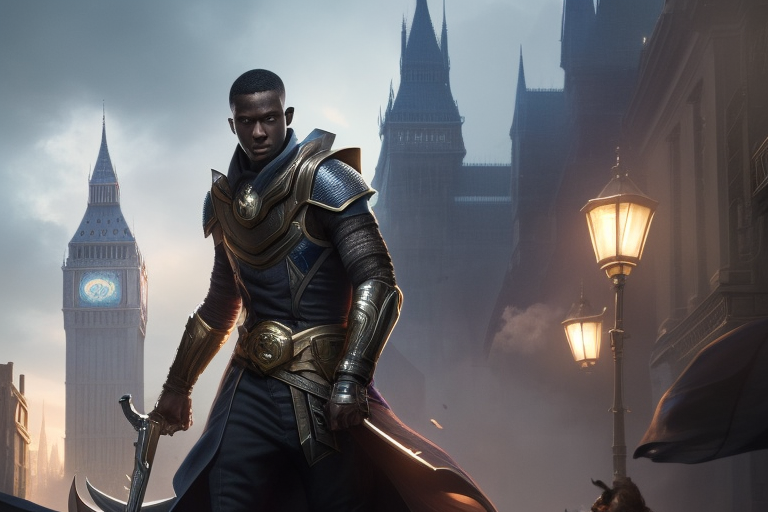
\includegraphics{a-skilled--assassin-ready-to-disappear-with-his-invisibility-cloak-he-is-a-young-black-man-he-is-a.png}
\caption{a-skilled--assassin-ready-to-disappear-with-his-invisibility-cloak-he-is-a-young-black-man-he-is-a.png}
\end{figure}

Hakram è un affascinante mezz'elfo con occhi vivaci, pelle e capelli
scuri. La sua agilità naturale è evidente in ogni movimento, e la sua
postura è sempre rilassata, pronto a sfuggire a qualsiasi situazione
pericolosa.

\subsection{2. Biografia}\label{biografia}

\begin{center}\rule{0.5\linewidth}{0.5pt}\end{center}

Cresciuto tra gli alberi dell'oscura Foresta dei Giganti da un vecchio
nano, Hakram non ha mai conosciuto i suoi genitori biologici. Dopo la
morte di suo padre adottivo, avvenuta quando aveva solo 14 anni, ha
imparato rapidamente le arti dell'inganno, del furto e della fuga,
diventando un abile ladro, girovago tra i villaggi e le città di
Valtara. Nonostante la sua vita criminale, ha un codice morale che gli
impedisce di fare del male a chi non se lo merita. Al momento nessuno sa
dove siano Hakram e Leona, ne se siano ancora vivi.

\subsection{3. Carriera}\label{carriera}

\begin{center}\rule{0.5\linewidth}{0.5pt}\end{center}

Dopo anni a vagare senza meta, Hakram si è stabilito nella capitale
Dishartiana, dove è diventato uno dei ladri più famosi per le sue
abilità di scasso e infiltrazione. È noto per i suoi colpi audaci e
sfuggenti, che gli hanno guadagnato rispetto tra i suoi compagni
criminali. La sua conoscenza dei luoghi e delle vie nascoste della
capitale dishartana è insuperabile, il che lo rende un compagno
inestimabile per qualsiasi colpo. L'imperatore ha messo sulla sua testa
una taglia di 10000 monete d'oro.

\subsection{4. Personalità}\label{personalituxe0}

\begin{center}\rule{0.5\linewidth}{0.5pt}\end{center}

Nonostante la sua professione, Hakram è un individuo affabile e
simpatico. Ha un senso dell'umorismo tagliente e sa come tranquillizzare
gli altri con la sua presenza rassicurante. È un romantico e ha un lato
gentile che riserva solo a coloro che hanno guadagnato la sua fiducia.
L'incontro con la principessa Leona ha trasformato la sua vita. Si è
innamorato profondamente di lei, e ora, con la notizia della prossima
paternità, è determinato a proteggere la principessa e il loro bambino
da qualsiasi minaccia che si profili all'orizzonte, in particolar modo
dalle responsabilità della corona. La sua abilità nel mondo dei ladri e
il suo sentimento d'amore lo hanno reso un partner devoto e pronto a
tutto.

\subsection{A. Coinvolgimenti in Eventi
Recenti}\label{a.-coinvolgimenti-in-eventi-recenti}

\begin{center}\rule{0.5\linewidth}{0.5pt}\end{center}

\href{Untitled\%20Database\%2049897c1ada034aeebc6c1efae06d3b26.csv}{Untitled
Database}
